\newpage
\section{Multiperiod Lot Sizing model}

% Introduzione
\subsection{Introduzione}
\hl{Discretiziamo il tempo} e quindi divido la pianificazione in \hl{slot di tempo} esistenti come ore, settimane, mesi. Avremo allora una \hl{domanda $d_t$} che fa rferimento al \hl{periodo $t=1,...,T$} con $T$ lunghezza dell'orizzonte di pianificazione.


\begin{figure}[H]
\centering
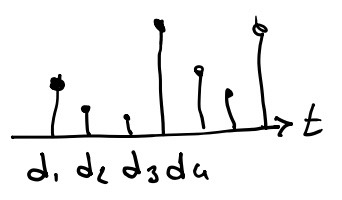
\includegraphics[scale=0.2]{discrettemp.jpeg}
\caption{Discretizzazione del tempo} 
\label{discrettemp}
\end{figure}


Dobbiamo definire:

\begin{enumerate}
    \item varaibili generali:
    \begin{itemize}
        \item \hl{$f_t$}: \textbf{costi fissi di produzione}, potrebbero dipendere dal periodo ma \textbf{non dipendono dalla quantità prodotta} (es: gas, elettricità)
        \item \hl{$c_t$}: \textbf{costi variabili} per la produzione di un prodotto, potrebbe dipendere dal periodo (es: vagetali)
        \item \hl{$h_t$}: \textbf{costi di stockaggio} per un periodo $t$
        \item \hl{Q}: \textbf{capacità di magazzino}
    \end{itemize}

    \item variabili decisionali:
    \begin{itemize}
        \item \hl{$y_t$}: \textbf{variabili di accenzione}
            $$y_t =
            \begin{cases} 
                = 1 \text{se è acceso} \\ 
                = 0 \text{se è spento}
            \end{cases}
            $$

        \item \hl{$x_t$}: indica la \textbf{produzione nel periodo $t$}
        \item \hl{$I_t$}: indica il \textbf{livello di scorte nel periodo $t$}
    \end{itemize}

    \item \hl{funzione obiettivo}:
        $$z = \text{ costi fissi } + \text{ costi variabili } + \text{ costi di inventario }$$
        $$z = \sum_{t=1}^T f_t y_t + \sum_{t=1}^T c_t x_t + \sum_{t=1}^T h_tI_t$$

    \item vincoli:
    \begin{itemize}
        \item \hl{di conservazione delle scorte}: cioè il livello di scorte a fino al periodo precedente e la merce prodotta, togliendo ciò che diamo al mercato:
            $$I_{t-1} + x_t + -d_t = I_t$$
        \item \hl{di capacita'}: dove \textbf{il livello di scorte non deve superare la capacità di magazzino}
            $$I_t \leq Q$$
        \item \hl{lega $x_t$ cno $y_t$}: \textbf{lega accenzione e spegnimento} dei macchinari
            $$x_t \leq (\sum_{i=t}^T) d_i\ \ \ \forall\ \ \ t=1,..,T$$

            essendo $y_t$ binaria, avremo:
            $$y_t =
            \begin{cases} 
                = 1 \to x_t\leq \sum_{i=t}^T d_i  \\ 
                = 0 \to x_t\leq 0\to x_t=0
            \end{cases}
            $$
        \item \hl{sull'inventario}: $I_0, I_T = 0$
        
    \end{itemize}
\end{enumerate}


% Aggiornamento il Beer Game - Backlog
\subsection{Aggiornamento Beer Game - Backlog}

In un problema reale \hl{non sono certo di soddisfare la domanda}, infatti si potrebbe andare \hl{sotto scorta} per cercare di soddisfarla con un \hl{incremento del costo}.
Il \hl{livello delle scorte si divide in una parte positiva ed una negativa}:  
$$I_t = I_t^+ -I_t^- \leq \geq 0$$

con $I_t^+$ livello di inventario e $I_t^-$ backlog.

avremo allora:
\begin{enumerate}
    \item \hl{funzione obiettivo}: 
        $$z = \sum_{t=1}^T f_t y_t + \sum_{t=1}^T c_t x_t + \sum_{t=1}^T h_tI_t^+ + \sum_{t=1}^T b_tI_t^-$$
    \item vincoli:
    \begin{itemize}
        \item \hl{di conservazione delle scorte}:
            $$I_{t-1}^+ - I_{t-1}^- + x_t - d_t = I_{t-1}^+ - I_{t-1}^-\ \ \ \forall\ \ \ t=1,...,T$$
        \item \hl{di capacita'}:
            $$I_t^+ \leq Q$$
        \item \hl{lega $x_t$ cno $y_t$}:
            $$x_t \leq (\sum_{i=t}^T) d_i\ \ \ \forall\ \ \ t=1,..,T$$
    \end{itemize}
\end{enumerate}


% Aggiornamento il Beer Game - Lead time 
\subsection{Aggiornamento Beer Game - Lead time $l\in\{0,1,2,...\}$}

Durante il \hl{periodo di arrivo degli ordini} le prime $l$ settimate non posso sperare di ricevere rifornimenti, infatti \hl{arrivera' nel periodo $t+l$}. Abbiamo i vincoli:

\begin{itemize}
    \item prime $l$ settimane: 
        $$I_{t-1}^+ - I_{t-1}^- - d_t = I_{t-1}^+ - I_{t-1}^-\ \ \ \forall\ \ \ t=1,...,l$$
    \item le altre settimane:
        $$I_{t-1}^+ - I_{t-1}^- + x_{t-l} - d_t = I_{t-1}^+ - I_{t-1}^-\ \ \ \forall\ \ \ t=l+1,...,T$$
\end{itemize}
